\selectlanguage{greek}
\chapter{Εισαγωγή}
\te{TODO:} --γενική εισαγωγή, ιστορική αναδρομή, χρησιμότητα--
\section{Το Πρόβλημα}
Τα συστήματα εντοπισμού θέσης (\te{localization systems}) είναι συστήματα
που έχουν τον γενικό στόχο να υπολογίσουν την θέση ενός αντικειμένου μέσα σε έναν δεδομένο χώρο.
Τα είδη του χώρου μπορούν να διαφέρουν σε διάφορες παραμέτρους. Το μέγεθος του χώρου μπορεί να είναι ένα δωμάτιο, μια πόλη ή μια ήπειρος ενώ το περιβάλλον του χώρου μπορεί να είναι αστικό ή υπεραστικό. Είναι προφανές πως κάθε περίπτωση απαιτεί μια διαφορετική προσέγγιση, για παράδειγμα ένα σύστημα παγκόσμιου εντοπισμού όπως το \te{GPS} δεν μπορεί να δουλέψει αποδοτικά σε έναν κλειστό χώρο για λόγους που θα αναλυθούν στη συνέχεια. Παρακάτω παρουσιάζουμε κάποια παραδείγματα διαφορετικών περιπτώσεων.
\subsection{Εποπτεία Ασφαλείας}
Η εποπτεία ασφαλείας είναι μια περίπτωση στην οποία ένας άνθρωπος που βρίσκεται απομονωμένος σε κάποιον
χώρο έχει λόγο να νιώθει πως η ασφάλεια του βρίσκεται σε κίνδυνο\cite{bernard}. Σε αυτήν την περίπτωση κάποιος
υπεύθυνος ασφαλείας μπορεί να ενημερώνεται ανα χρονικά διαστήματα για την τοποθεσία του εν λόγω ανθρώπου μέσο του κινητού
τηλεφώνου του, χρησιμοποιώντας τεχνικές εύρεσης τοποθεσίας. \\~\\
Σε τέτοιες περιπτώσεις συνήθως υπάρχει και μια λειτουργία έκτακτης ανάγκης, η οποία αμέσως υπολογίζει την τοποθεσία του κινητού τηλεφώνου και την εμφανίζει στον υπεύθηνο ασφαλείας\cite{bernard}.
\subsection{Ρομπτοτικός Έλεγχος}
Στην περίπτωση ρομποτικού ελέγχου μπορούν να εφαρμοστούν πιο προηγμένες τεχνικές εντοπισμού εσωτερικού χώρου
απο ο,τι τεχνικές μπορούν να εφαρμοστούν, για παράδειγμα, σε ένα απλό κινητό, καθώς δεν υπάρχουν οι ίδιοι τεχνολογικοί και πρακτική περιορισμοί.
Ο έλεγχος των ρομπότ γίνεται με αυτοματοποιημένους κανόνες που βασίζονται στην τοποθεσία τους\cite{bernard}, σε περιβάλλοντα όπως αποθήκες.
\begin{figure}[h]
\centering
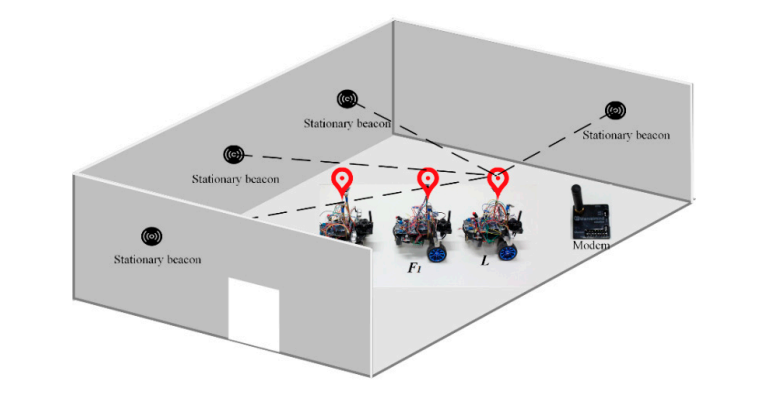
\includegraphics[width=10cm]{pictures/robot_IPS.png}
\caption{Σύστημα Εντοπισμού για Ρομποτικές Εφαρμογές\cite{honganyang}}
\end{figure}

\subsection{Πολυκαταστήματα}
Στην περίπτωση των πολυκαταστημάτων, οι ιδιαίτερεα μεγάλοι και πολύπλοκα διατεταγμένοι χώροι χρήζουν την χρήση συστημάτων εντοπισμού\cite{spinclabs}. Το κινητό τηλέφωνο του πελάτη ή μια ειδική συσκευή που δίνεται κατα την είσοδο στο κατάστημα χρησιμοποιείται για την εντόπιση του πελάτη μέσα στον χώρο, και κατ'επέκταση την καθοδήγηση του, πρός τους διαδρόμους και τα προϊόντα που θέλει. Ταυτόχρονα τα δεδομένα που συλλέγονται απο τις κινήσεις των πελατών είναι χρήσιμα για το κατάστημα ως προς την χωροταξία του.
